\documentclass[11pt,a4paper,twocolumn]{scrartcl}

% Support for UTF-8 and non-English letters require the following two
\usepackage[T1]{fontenc}
\usepackage[utf8]{inputenc}
\usepackage{algorithm2e}
\usepackage{fancyvrb}
% Font packages
\usepackage[default,defaultsans,oldstyle,proportional]{lato}
\usepackage[scaled]{beramono}
\usepackage{sfmath}
% Optimized justification via improved microtypography on character level
\usepackage{microtype}
\usepackage{ragged2e}
\usepackage[none]{hyphenat} % disable all hyphenation
\setlength{\emergencystretch}{3em} % allow extra hfill, needed if hyphenation disabled
%\overfullrule=1mm % mark overfull boxes
%\usepackage{showframe} % show edges of text areas
% Page layout
\usepackage[left=15mm,right=15mm,top=15mm,bottom=20mm,
   nohead,foot=10mm]{geometry}
% Page headers
\usepackage{scrlayer-scrpage}
\usepackage{lastpage}
% Page header
\KOMAoptions{headsepline=0pt,plainheadsepline=off}
\ihead*{}
\chead*{}
\ohead*{}
% Page footer
\KOMAoptions{footsepline=0pt,plainfootsepline=off}
\ifoot*{}
\cfoot*{Page \thepage{} of \pageref*{LastPage}}
\ofoot*{}
% Text layout
\KOMAoption{parskip}{never}
\newlength{\myparindent}
\newlength{\myparskip}
\setlength{\myparindent}{0pt}
\setlength{\myparskip}{5pt plus 1pt}
\setparsizes{\myparindent}{\myparskip}{0.1\linewidth plus 1fil}
\RedeclareSectionCommand[beforeskip=6pt,afterskip=3pt,afterindent=false]{section}
\RedeclareSectionCommand[beforeskip=6pt,afterskip=-0.5em,afterindent=false]{paragraph}
\RaggedRight
% SVN metadata
\usepackage[today,revrange,nofancy]{svninfo}
\svnInfo $Id$
% Graphics
\usepackage{graphicx}
% Colour definitions
\usepackage{xcolor}
\definecolor{secondary}{HTML}{435584}
% Floats
\usepackage{subcaption}
% Listings
\usepackage{listings}
\lstset{language=C, basicstyle=\small\ttfamily,
   aboveskip=0pt, belowskip=0pt}
\usepackage{upquote} % to use correct glyphs for single-quote in verbatim
% SI units
\usepackage{siunitx}
\sisetup{per-mode = symbol, detect-all = true}
% Hyperlinks
\usepackage[
   colorlinks=true,allcolors=secondary,breaklinks=true,
   bookmarks=true,unicode=true,bookmarksopen,bookmarksnumbered]{hyperref}
\usepackage{multicol}

% Document-specific settings
\renewcommand\abstractname{Executive Summary}

% define a critical section block
\SetKwBlock{CritSection}{critical section}{}

% Document details
\title{Design Brief: Group 5}
\author{
   Gabriel Apap,
   Damjan Filipovic,
   Mark Mizzi
   }
\date{\svnMaxToday, Document v.\svnInfoMaxRevision}

\begin{document}

\maketitle

\abstract{%
   This document outlines the design of a DTMF encoding system based on a microcontroller board. The system described makes use of an LCD display to show the user what keys they have pressed as well as to display any messages or errors. An LED is used as an indicator of the system's state. An on-board DAC, in conjunction with an amplifier circuit and speaker are used to generate and amplify the DTMF tones.
   }

\section{Introduction}

   Dual Tone Multi Frequency (DTMF for short) encoding is a technology used to communicate with other devices over a standard analogue telephone line \cite{sl:an218}. This is mainly used for automated switchboards for calls; however, this is also used in remote control systems, telephone banking, and other applications \cite{sl:an218}.

   The technology functions by converting each of the 16 symbols on a keypad (1-9, A-D, * and \#) into a specific tone. The tone consists of a sum of two sine waves, whose frequency is determined by pairwise combination of 4 high frequencies (representing the keypad columns) and 4 low frequencies (representing the keypad rows) \cite{sl:an218}.

   The goal of this project is to implement a DTMF encoding system based on the Embedded Artists LPC4088 microcontroller board.

   Microcontrollers are designed for use in real-time systems, and hence do not have an operating system which deals with the issue of task management. Task scheduling has to be handled explicitly by the programmer, through the use of an ad-hoc scheduler and/or interrupt handlers.

   In addition, microcontrollers are generally low-cost systems with limited hardware resources, and hence require the use of low-level programming tricks to achieve efficiency and performance despite the resource constraints.
   
   The DTMF system implemented will make use of several I/O devices, including an LCD used to convey user input or settings options to the user,
   an indicator LED which turns on when the system is booted, and a keypad input device used to choose between settings or to input DTMF symbols.

   On boot-up, the system will prompt the user to enter one of two operational modes: settings or normal mode.

   In settings mode, the user is presented with numbered options which can be used to configure the system. 
   The user's options are persisted to flash memory for use in normal mode.
   The options available to the user will include:

   \begin{enumerate}
      \item Inter-symbol spacing, i.e. the delay between two consecutive tones being produced.
      \item Symbol length, i.e. the duration for which a single tone is produced.
      \item Tone resolution. This setting affects the sampling frequency of the tone produced.
      \item Reboot system. This saves the chosen options and resets the system.
   \end{enumerate}

   When the system enters normal mode, options are loaded from flash memory, and the system behaves as a DTMF encoder, 
   producing tones when the user presses keys.

   Section \ref{system-design} describes the proposed design for the DTMF encoding system. The system's architecture is described in subsection \ref{system-arch}. 
   Subsection \ref{polling-method} clarifies some implementation details regarding the keypad input.

   Section \ref{schedule} outlines a breakdown of the system's implementation into individual tasks, as well as a schedule for implementing these tasks.

\section{System Design} \label{system-design}

\subsection{System architecture} \label{system-arch}

To implement these features while adhering to good seperation of concerns, the system must make use of several software components.
The proposed software components are shown in Figure \ref{fig:software_components}.

\begin{figure*}
   \centering
   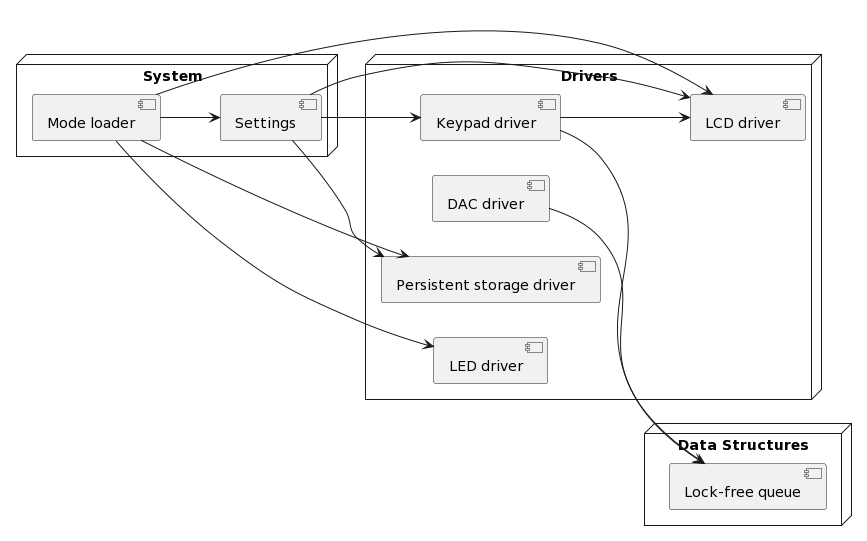
\includegraphics[width=0.92\textwidth]{software_components}
   \caption{Software components proposed for the system, grouped by functionality. Arrows between components indicate caller-callee dependencies.}
   \label{fig:software_components}
\end{figure*}

Not shown in this figure is the use of several global variables to store the state of the system. These include 
(i) a thread-safe flag which indicates whether a tone is being generated,
(ii) a counter used to keep track of tone generation in between interrupt handler invocations,
(iii) a read-only lookup-table containing samples of the $\sin$ function, and
(iii) a \verb!struct! holding user configuration of the system.

It is also worth noting that the lock-free queue indicated in the design is globally allocated, and is accessed by several ``threads'' of execution.

The responsibilities and features of each of the software components indicated in the figure will now be described.

The \textbf{mode loader} is the entry point of the system. It turns on the indicator LED, and presents the user with options for choosing between settings mode or normal mode. It must also process any key press which indicates the user's choice, and load the code for settings or normal mode (through a function call).

The \textbf{settings} component will contain the code for settings mode. It must present the user with options for configuring the system, and process the user's choice. When the user chooses to re-boot the system, it must also persist the chosen configuration to flash memory.

The \textbf{DAC driver} is central to system operation, as it contains functions which generate the DTMF tones. The module should provide a function which, 
given a symbol, enables a timer interrupt handler (depending on what tone is to be produced) and sets the timer duration to the sampling frequency of the tone.

The module should also implement 16 timer interrupt handlers (one for each tone) to produce tone samples and drive the DAC. The interrupt handlers will be similar in behaviour, and will share a lot of their code. The benefits of having an interrupt handler for each tone is that it reduces the amount of global state used by the system and allows the compiler to aggressively optimize the handlers in question, e.g. applying constant division optimization.

The behaviour of each interrupt handler is shown in the control flow diagram in Figure \ref{fig:tone_interrupt_cfd}.

\begin{figure*}
   \centering
   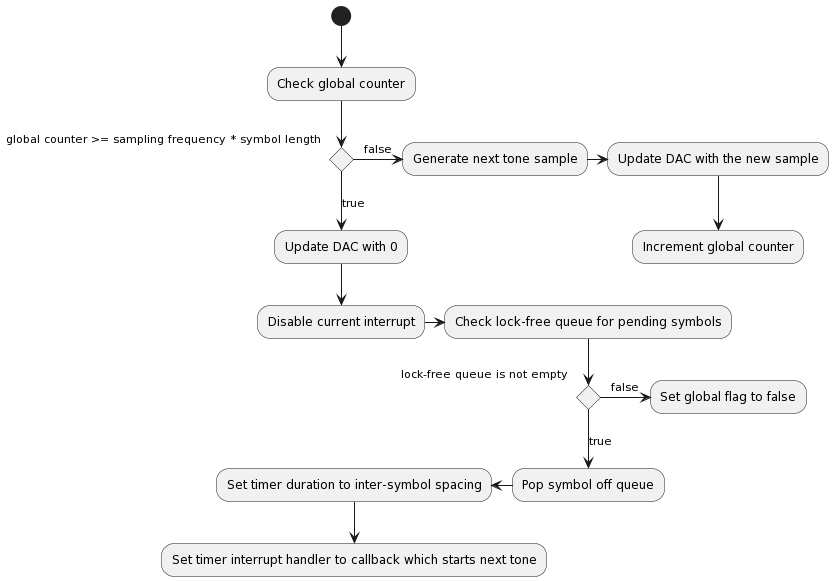
\includegraphics[width=0.92\textwidth]{tone_interrupt_cfd}
   \caption{Control flow diagram illustrating behaviour of tone-generating interrupt handlers}
   \label{fig:tone_interrupt_cfd}
\end{figure*}

The \textbf{keypad driver} component provides an abstraction layer over the keypad. It must implement a single polling cycle (as a function) for use in other modules.

In addition, it must implement a method that whilst running the polling cycle, performs the following actions immediately on detection of a key press:
\begin{enumerate}
   \item It immediately outputs the DTMF symbol detected to the LCD screen.
   \item It checks if there is a tone interrupt handler enabled. This can be done by atomic test and set on the global flag.
   \item If there is no tone interrupt handler enabled, it takes the symbol detected, and enables a tone-generating interrupt handler to generate its tone 
      (using a method in the DAC driver).
   \item If there is already a tone interrupt handler enabled, it pushes the DTMF symbol onto the output queue.
\end{enumerate}
This method will be used in normal mode to process key presses.

The \textbf{persistent storage driver} provides an abstraction layer over the flash memory. It provides functions to serialize and deserialize the C structs 
which need to be stored into a byte stream, and allows for loading or storing serialized data from/to flash memory. The use of a wear leveling algorithm when storing data is essential to prevent the flash memory from degrading quickly\cite{silberschatz2018operating}.

The \textbf{LED driver} provides methods to turn the indicator LED on or off.

The \textbf{LCD driver} provides an abstraction layer over the LCD screen. It must implement methods which allow a DTMF symbol or a C string to be encoded and
displayed on the LCD.

The \textbf{lock-free queue} is a globally allocated thread-safe data structure. It needs to support the following thread-safe (atomic) operations:
\begin{enumerate}
   \item Enqueue a DTMF symbol.
   \item Check if queue is empty and dequeue. This must be one atomic operation.
\end{enumerate}

\subsection{Implementation of the lock-free queue}

Several simplifying assumptions about the system can be made in implementing the queue.

Firstly, since the queue is filled from user input, it can be assumed that the system will on average consume elements from the queue much faster than they are produced. For this reason, a fixed size queue is acceptable, so long as the size makes it hard for a user to overflow the queue. Appropriate error handling can be used to deal with an overflow situation (for e.g. by resetting the system).

This assumption allows us to implement the queue as a circularly indexed array, rather than a more complex linked list data structure. A size of 4096 elements was chosen.

Although this implementation approach significantly simplifies code, and may also be more performant than a linked list approach (which would resort to a \verb!malloc! implementation for allocating nodes), one downside is that the queue takes up a significant portion of memory, while being mostly under-utilized.

Secondly the system only involves one consumer (the DAC interrupt handler), and one producer (the input processing loop). For this reason, the lock-free queue can be implemented using just a single shared variable $N$, which is the size of the queue. The variables holding indices of the queue's head and tail can be considered unshared.

Pseudo-code for the queue's operations is presented in Algorithms \ref{alg:enqueue} and \ref{alg:check_dequeue}.

\begin{algorithm}
   \caption{Pseudocode for the lock-free queue's enqueue operation. Note the atomic increment of $N$}\label{alg:enqueue}
   \KwData{
      \begin{itemize}
         \item $q$ is the queue array
         \item $tail$ is the immediate index after the last element in the queue
         \item $s$ is the symbol to be enqueued
         \item $N$ is the number of items in the queue
         \item $M$ is the queue size (maximum capacity of the queue)
      \end{itemize}}
      \textbf{atomic} $N \gets (N + 1) \bmod M$; \\
      $q[tail] \gets s$; \\
      $tail \gets (tail + 1) \bmod M$;
\end{algorithm}

\begin{algorithm}
   \caption{Pseudocode for the lock-free queue's check and dequeue operation.}\label{alg:check_dequeue}
   \KwData{
      \begin{itemize}
         \item $q$ is the queue array
         \item $head$ is the index of the start of the queue
         \item $N$ is the number of items in the queue
         \item $M$ is the queue size (maximum capacity of the queue)
      \end{itemize}}
      \CritSection{
         $tmp \gets N$;\\
         \If{$tmp = 0$}
         {
             $N \gets (tmp - 1) \bmod M$\;
         }
      }
      $res \gets default$;\\
      \If{$tmp \ne 0$}
      {
         $res \gets q[head]$;\\
         $head \gets (head + 1) \bmod M$;
      }
\end{algorithm}

Both the atomic increment in enqueue, and the critical section in check and dequeue can be implemented using hardware synchronization. The ARMv7-M architecture provides \verb!LDREX! (load exclusive) and \verb!STREX! (store exclusive) instructions.

When a load exclusive instruction is used, a hardware monitor tracks subsequent stores to a small block containing the loaded address using a tag. Once a single exclusive store to the block has been executed, the monitor prevents subsequent exclusive stores before another exclusive load is performed.\cite{armv7_m_architecture_manual}

\subsection{How the polling method is invoked} \label{polling-method}

There are several ways in which the polling cycle procedure that processes user input in normal mode (described above) can be executed.

The simplest method is to run the procedure in application mode, with a set period of busy waiting in between invocations of the method to avoid spurious input.
(A human user will keep a key pressed for several clock cycles.)

A more sophisticated option is to run the procedure as an interrupt handler for a timer interrupt, with the timer duration set to avoid spurious input. In this version, the processor has no application code to run and can be put in sleep mode in between interrupt invocations. While more efficient than the busy-waiting approach, this method can still invoke the interrupt handler when there is no input to process.

A final, more efficient approach is to have a keypad-driven interrupt handler. In this approach, the columns of the keypad are set high, and pressing any key
triggers a pin interrupt for its row. The interrupt handler then invokes the polling method to find which key in that row was pressed and handle it.

Each of these design choices is more sophisticated than the last, while re-using much of the same code. The plan is to implement each of these designs in turn. When one implementation has been successfully tested, the team will move on to implementing a more sophisticated design.

\section{Management} \label{schedule}
\subsection{Final Deadline}
The final deadline will be set to \textbf{10\textsuperscript{th} May} to ensure that the work is done at a proper pace whilst leaving enough room for any necessary 
adjustments.

\subsection{Tasks}
To implement the system, the above-mentioned software components have to be split into multiple sub-tasks. Each task will have a fairly allocated time-frame for completion. The deadlines for each task are as follows:
\subsubsection{Drivers}
\begin{enumerate}
    \item LCD Driver - Deadline: \textbf{8\textsuperscript{th} April}. Subtasks: Symbol and C-String to LCD function, Display function.
    \item Keypad Driver - Deadline: \textbf{8\textsuperscript{th} April}. Subtasks: Polling Cycle function for the keypad, Keypad driven interrupt.
    \item LED Driver - Deadline: \textbf{8\textsuperscript{th} April}. Subtasks: LED On function, LED Off function.
    \item Persistent Storage Driver - Deadline: \textbf{16\textsuperscript{th} April}. Subtasks: Serialising Data, Persisting Data, Loading Data, Deserializing Data.
    \item DAC Driver - Deadline: \textbf{20\textsuperscript{th} April}. Subtasks: Timer interrupt handler enable method, Set timer duration function, Interrupt handlers.
\end{enumerate}

\subsubsection{Data Structures}
\begin{enumerate}
    \item Lock-Free queue - Deadline: \textbf{1\textsuperscript{st} April}. Subtasks: Atomic Enqueue function, Atomic Check and Dequeue function.
\end{enumerate}

\subsubsection{System}
\begin{enumerate}
    \item Mode loader - Deadline: \textbf{16\textsuperscript{th} April}. Subtasks: Display Options function, Load settings/normal mode functions.
    \item Settings Mode - Deadline: \textbf{27\textsuperscript{th} April}. Subtasks: Display settings function, Save settings function.
\end{enumerate}

\subsection{Task Dependencies}
When considering the inter-dependencies of the tasks listed above, there is a discrete order of task development that when followed should ensure that each subsequent task has adequate resources to be accomplished. The order is the following:
\begin{enumerate}
    \item Lock-Free Queue
    \item LCD Driver
   \item LED Driver
   \item Keypad Driver
   \item Persistent Storage Driver
   \item DAC Driver
\end{enumerate}

\section{Closure}

In conclusion, this document describes the design of an efficient and performant system implementing DTMF encoding. The system's software has been split up
into several modules showing good separation of concerns. Although not discussed here, a highly efficient algorithm has been derived for use in tone generation.

\bibliographystyle{ieeetr}
\bibliography{references}

\end{document}
